\chapter{System Design}
\label{ch:system-design}
\graphicspath{{./img/system-design/}}

In this section the block level system design is done and the direction finding algorithm decided on.
The design is done based on the user requirements specified in \Cref{ch:introduction} as well as the data and background gathered in \Cref{ch:lit-review}.
Once the system is designed, some simulations are run to show whether the algorithm performs as expected and also to highlight potential problems that need to be tackled.

\section{Sub-systems}
The DF system will consist of the following sub-systems.
A block diagram view of what's been described here is shown in \Cref{fig:system-design:signal-flow} with some additional requirements noted.

\subsection{Antenna Array}
The antenna array will receive the RFI signals. The user requirements state that a \SI{360}{\degree} field of view is necessary. Hence, a circular array will be used. The arrays needs to be useful in direction finding both narrow band and impulsive signals. This implies that a trade-off will have to be made in terms of element spacing when designing the array. If the element spacing is too large, the array will experience high amounts of phase ambiguity and perform poorly at narrow band DF. If the element spacing is too small the time difference for impulsive signals will be difficult to measure. The elements should be non-dispersive to facilitate keeping the structure of the impulsive signals. The number of elements to be used in the array will be explored later.

\subsection{Front End}
The front end will contain anti-aliasing filters and low noise amplifiers. For this project, a simple front end will be used. There will be no mixing or switching: the base band signal will be low pass filtered and amplified. The specifications of the filters and amplifiers will be specified based on the operating frequency band of the array and the sampling frequency of the ADCs. There will need to be an independent, identical RF chain for each element of the array.

\subsection{ROACH}
The ROACH board will have the functions of doing analogue to digital conversion and the high-speed digital signal processing. The ROACH consists of a Virtex 5 FPGA and multiple ADC cards allowing all of the RF inputs will be digitsed independently. The purpose of the ROACH is to do real-time processing on the raw ADC samples, hence reducing the data rate to only signals of interest which can be sent to the computer and processed there.

\subsection{Computer Software}
The computer will receive input from the ROACH and do further DSP. Specifically, the final angle of arrival estimation. The computer needs to be able to log all of the data for future analysis and display the results of the direction finding to the user real-time in the field.


\begin{landscape}
  \thispagestyle{empty}
  \begin{figure}
    \centering
    \makebox[\textwidth][c] {
      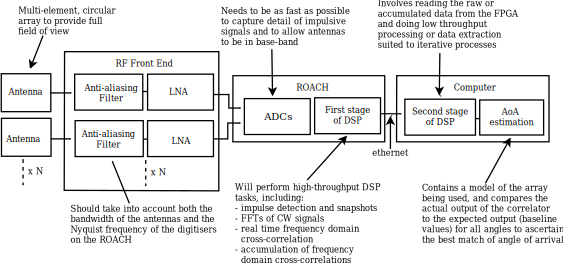
\includegraphics[width=\paperwidth, clip=true, trim = 80 500 80 80]{basic-flow}
      % left, bottom, right, top
    }
  \caption{Block diagram view of the flow of signals through the proposed direction finding system. The key function of the blocks has been noted on the diagram. }
  \label{fig:system-design:signal-flow}
  \end{figure}
\end{landscape}

\section{Direction Finding Algorithms}
With the above blocks available, this section goes into selecting an appropriate direction finding algorithm which meets the user requirements and refining what will be done in the first and second stage of DSP. Some additional requirements for the other blocks that arise from the selected algorithm are noted. 

This section details how the selected finding algorithm will be implemented on the system. Following will be a simulation of the algorithm and the system in operation is written in python and the output of this simulation is shown here, demonstrating that the algorithm is capable of carrying out the task.\\

There are two cases that the algorithm needs to deal with: weak narrow band signals and strong impulsive ones. The narrow band case naturally lends itself to frequency domain analysis, since the information about narrow band continuous signals is easily expressed in the frequency domain. The impulsive signals, however, are more naturally dealt with in the time domain as they are clearly bounded in time, existing only for a short duration, while being spread all over the frequency domain. 

As such, the selected algorithm contains two distinct parts: a phase interferometry component designed to direction find weak (below the noise floor) narrow band signals, and time difference of arrival part designed to locate strong (noticeable when plotted when plotted in the time domain) short duration impulsive RFI.

\subsection{Phase Interferometry}
Phase Interferometry direction finding of narrow band signals will be done by phase comparison of the signal of interest as seen by each antenna in the array. The technique of phase interferometry has been extensively explored in the literature review. The process carried out by this DF system will be as follows.
\begin{enumerate}
  \item Use ADCs to sample the signal seen by each antenna exactly in phase. The ADCs need to be calibrated and have equal cable length to each antenna.
  \item Stream the output of each ADC into a real-time FFT which is capable of producing Fourier transforms of the observed signals as fast as they are captured. The FFTs must stream their frequency channel outputs at the same data rate that they get time domain data in.
  \item Do a cross correlation between each pair of antennas (baselines). In the discrete frequency domain this means multiplying the value of each frequency channel from one antenna by the complex conjugate of the value of the corresponding frequency channels from another antenna. The output of this complex conjugate multiplication is a spectrum where the phase of each channel is the phase difference of the two input spectra. The amplitude of the channel is simply the product of the two input amplitudes, but it's not that important for this application.
  \item For weak signals, the phase of the cross correlation spectrum may be dominated by noise. Attempting to read off phase difference from the output of a single FFT would probably not work as the phase would be dominated with noise. However, assuming we've got Gaussian white noise, the noise component should average to zero. Taking advantage of this we can add multiple of these cross correlation spectra together. The signal component (phase difference of a baseline) will sum coherently while the noise component will sum to zero. As such, the more spectra are summed the more the signal component will stand out of the noise.
  \item After sufficient spectra have been summed, take a snapshot of the result and extract the phase from the frequency channel of interest from each baseline spectra. Construct a \(N\)-dimensional vector of these observed baseline frequency differences,e where \(N\) is the number of baselines.
  \item Construct a \(N \times M\) matrix where each column of the matrix is a vector of theoretical baseline time differences for the AoA corresponding to that column. This is essentially a sampled antenna array manifold. Here \(M\) is the number of sample angles which the manifold is calculated for. It can be made as large as one wishes. A larger \(M\) means a higher resolution AoA estimation at the cost of more computational complexity.
  \item For each column in the calculated manifold matrix, calculate the RMS error between the observed vector and that column. The column with the lowest RMS error is selected as the AoA of the signal. A measure of confidence can be given from the error.
\end{enumerate}

\subsection{Time Domain Direction Finding}
This technique is remarkably similar to the phase interferometry technique in that we are still capturing time domain signals from the antenna using ADCs which are sampling in phase, measuring a parameter of the received signal from the array, comparing it to the theoretical response from the array at every angle and finding the angle whose expected output most closely matches the measured signal. Hence much of the process described above will still apply.

The key difference is that instead of the parameter of interest being the phase difference of a frequency channel, the parameter of interest is the time difference of the signal at each antenna. As such it's necessary to capture time domain snapshots of the signals seen be each antenna and do time domain cross correlation to find the time domain offset of the signal seen by each antenna. The peak of the cross correlation output corresponds to the time difference. Strictly speaking it's actually the ADC clock sample difference, but seeing as the ADC is being clocked at a known rate that can easily be converted to time difference. The antenna array manifold constructed will be in the time domain rather than the frequency domain.

Additionally, as the time domain cross correlation process is computationally expensive, it will only be done when a signal is detected. This implies than an impulse detector of some sort must be present and must be able to trigger the DF process

\subsubsection{Upsampling for resolution}
For the impulsive signals which the time domain DF will be used for, there is no issue of ambiguity as the signals are not periodic like continuous narrow band signals are. Instead, the issue is one of resolution. In order to get accurate time difference readings, a high time resolution snapshot of the signals must be taken. This means a fast ADC. The higher the time resolution of the signal, the more cross correlation points there are and the greater the accuracy of the time domain measurement.

Fortunately we can use upsampling to increase the resolution of the time domain cross correlation provided some requirements are met, and at the expense of additional computational complexity. The computational complexity comes both from the upsampling process as well as from the increased number of datapoints in the cross correlation step.

The primary requirement is that we've got a band limited signal with no unwanted aliasing happening. The system designed here is operating with base band sampling which implies that provided a suitable low-pass filter is used in accordance with the Nyquist–Shannon sampling theorem this will be met. Sampling like this means that we've got all of the information about the signal captured in the samples. As the signal is fully defined, smooth lines can be drawn between the sampled points. This means that new higher resolution samples can be taken by interpolating more points between the sampled points.

This technique of upsampling will be used to compensate for the fact that we'll be using a relatively small array, not typically suited to time domain direction finding. A small array has a lower time resolution which is good for limiting phase ambiguity for frequency domain direction finding but will produce an unusably low time domain resolution unless upsampled.

\section{Algorithm Simulations}
\subsection{Frequency Domain Simulations}
In preparation for the implementation of the DF algorithms, a Python package called directionFinder-backend was written. This package has the code for an AntennaArray class which builds an array model out Antenna objects. It can calculate and return a vector of the antenna array manifold.

An additional package, phase-ambiguity, has logic for creating an AntennaArray object and then correlating the manifold vector from a reference direction to manifold vectors from all directions to find matches and plot the results.

The phase ambiguity simulator takes in parameters of frequency range, number of discrete frequency points, simulated AoA range, number of angle points, and reference angle.
This produces a 3-d plot with axes for AoA, comparison angle and RMS error. Typically the 3-d plot is flattened to a 2-D image with colour used for the third dimension, rather than rendering a 3-d image. The type of data being plotted naturally lends itself to a colour plot view.


Ideally we would like 4 dimensional vectors: frequency, reference angle, aoa, correlation. However, this is difficult to do. Hence, two simulation strategies are used: either fix reference angle and vary frequency and AoA. Or fix frequency and vary reference and AoA. They produce results with a different view: one shows the ambiguity performance and a certain frequency, the other view shows the slice of the ambiguity performance over the whole frequency range. Process:

\subsubsection{Ambiguity Simulation Results}
The following plots are of array ambiguity for antenna arrays ranging from 3 to 9 elements. As the number of elements increases the array radius is increased linearly to ensure element spacing is maintained.

The simulation is for an signal arriving from \SI{0}{\degree}, and comparing how similar signals from other angles look to the system. This is a theoretical performance for a perfect signal in no noise. The ideal performance is that the signals from all angles other than \SI{0}{\degree} have a distinguishable phase difference. Two observations are made:
\begin{enumerate}
  \item Array with even number of elements suffer more from ambiguity than odd numbered arrays. This is due to there being line of symmetry in even numbered circular arrays.
  \item In general, the more elements you have, the lower the ambiguity. This is due to more baselines being able to resolve ambiguity.
\end{enumerate}

\begin{figure}[H]
  \centering
  \begin{subfigure}{0.95\textwidth}
    \centering
    \includegraphics[width=\textwidth, clip=true, trim = 10 15 53 0]{ambiguity03}
    % left, bottom, right, top
  \end{subfigure}\\[1em]
  \begin{subfigure}{\textwidth}
    \centering
    \includegraphics[width=\textwidth, clip=true, trim = 10 15 53 0]{ambiguity04}
  \end{subfigure}\\[1em]
  \begin{subfigure}{\textwidth}
    \centering
    \includegraphics[width=\textwidth, clip=true, trim = 10 15 53 0]{ambiguity05}
  \end{subfigure}
  \caption{Ambiguity plots for various antenna array sizes with reference signal arriving at \SI{0}{\degree}.}
\end{figure}
\begin{figure}[H]
  \ContinuedFloat
  \centering
  \begin{subfigure}{0.95\textwidth}
    \centering
    \includegraphics[width=\textwidth, clip=true, trim = 10 15 53 0]{ambiguity06}
    % left, bottom, right, top
  \end{subfigure}\\[1em]
  \begin{subfigure}{\textwidth}
    \centering
    \includegraphics[width=\textwidth, clip=true, trim = 10 15 53 0]{ambiguity07}
  \end{subfigure}\\[1em]
  \begin{subfigure}{\textwidth}
    \centering
    \includegraphics[width=\textwidth, clip=true, trim = 10 15 53 0]{ambiguity09}
  \end{subfigure}
  \caption{(cont'd) Ambiguity plots for various antenna array sizes with reference signal arriving at \SI{0}{\degree}.}
\end{figure}

\subsubsection{Accumulation Gain Simulation Results}

The other performance criteria of the frequency domain system is the ability to see weak signals below the noise floor. The contention is that by accumulating many datapoints, the noise component will sum to zero while the signal component will sum coherently.

To verify this, the simulation package was extended to add coherent noise at configurable SNR levels. Datapoints were generated and added, measuring the phase error after each datapoint. The result is show in \Cref{fig:system-design-integration-vs-error}. This demonstrates that the more datapoints are accumulated the lower the error. It also shows that the higher the SNR, the faster the error drops off.

\begin{figure}
  \centering
  \includegraphics[width=0.9\textwidth]{integration-vs-error-combined-5}
  \caption{Number of accumulations vs output SNR for various input SNR levels}
  \label{fig:system-design-integration-vs-error}
\end{figure}

This figure also demonstrates why it is difficult to quantify the performance of a DF system with a single "accuracy" number: the error is dependant on many factors, such as number of antenna elements, RFI signal strength and observation length.

\subsection{Time Domain Simulations}
The time domain system does not need either ambiguity or accumulations length measurements. The reason is that it does not suffer from ambiguity, and accumulation is not done for impulsive signals. What it does do, however, is upsampling. Quick simulation of Fourier method upsampling is done here to show how it works in principal. The Fourier method, also known as interpolation involves taking the Fourier transform of the received impulsive signal, zero pad the DTFT with a \(N \times M\) zeros where \(N\) is the length of the observed signal and \(M\) is the number of interpolated data points required, then inverse Fourier transform the signal back to the time domain. It is legal to zero pad a Frequency domain signal provided the received signal does not have any out-of-band or aliased components. This can be ensured with good analogue filtering.

It is worth noting that this interpolation can be done either on the raw signals or equivalently on the output of the cross correlation. This is important as there will be significantly less computation involved in interpolating the output of the cross correlation than the raw time domain signals. The reason is that correlation is only done over a small window of the raw signal, not over the whole signal.\\

An example is shown in \Cref{fig:system-design-raw-vs-upsampled-timedomain}. Here, the red signal with few datapoints is the original output of the time domain cross correlation. There is a clear peak data point in red, however the data point to the left is higher, implying that the real, continuous signal's peak is probably more to the left of the observed peak. When an upsampling is done and plotted in blue, the peak of the interpolated signal is more what would be expected.

\begin{figure}
  \centering
  \includegraphics[width=0.9\textwidth]{time-domain-cross-raw-vs-upped}
  \caption{Original cross correlation output with upsampled version overlaid. The upsampled version has a more accurate peak}
  \label{fig:system-design-raw-vs-upsampled-timedomain}
\end{figure}

\section{Summary}
This chapter has shown how a system with a circular antenna array, an RF front end, digitisers and DSP can be used to DF both narrow band and impulsive DF. It's been shown how antenna geometry impacts ambiguity performance, how accumulation can allow us to see below the noise floor, and how interpolation can be used to increase resolution of a band limited signal.
